\documentclass[12pt,a4paper]{article}
\usepackage{amsmath}
\usepackage{amssymb}
\usepackage{graphicx}
\usepackage{bm}

\topmargin  -18mm    
\textheight 254mm   
\textwidth 169mm    
\oddsidemargin -4mm
\begin{document}
\begin{center}
{\large \textbf{Approximating functions with cubic singularities}}\\
{\footnotesize \today}
\end{center}

\noindent To approximate functions of the form
\begin{equation}
f(\sqrt[3]{t^2 + \epsilon^2},t), \qquad t \in [-1, 1], \label{eq:algsingfun}
\end{equation}
we set $y = t$ and recast $f$ as a bivariate function $f(x,y)$ on the cubic curve $\gamma$, where
\begin{equation}
\gamma = \left\lbrace (x,y) \; : \; y^2 = \phi(x) = x^3 - \epsilon^2,\qquad y\in [-1, 1], \qquad x \in [\epsilon^{2/3}, \left(1 + \epsilon^2\right)^{1/3}] \right\rbrace, \label{eq:gammadef}
\end{equation}
and find its interpolant on $\gamma$. Let $(x_{k,N},\pm y_{k,N}), k = 1, \ldots, N$ be $2N$ points on $\gamma$, where $y_{k,N} = \sqrt{\phi(x_{k,N})} \neq 0$, then from Theorem~3.2, the unique interpolant of $f$ at the points $(x_{k,N},\pm y_{k,N}), k = 1, \ldots, N$ is
\[
L_N(f_e(x)) + yL_N(f_o(x)),
\]  
where 
\[
f_e = \frac{1}{2}\left[ f(x,\sqrt{\phi(x)}) + f(x,-\sqrt{\phi(x)}) \right], \qquad
f_o = \frac{1}{2\sqrt{\phi(x)}}\left[ f(x,\sqrt{\phi(x)}) - f(x,-\sqrt{\phi(x)}) \right],
\]
and $L_N(f_e(x))$, $L_N(f_o(x))$ are the Lagrange interpolating polynomials of $f_e$ and $f_o$ at $x_{k,N}, k = 1, \ldots, N$. 

For comparison purposes with standard bases, we also approximate functions of the form (\ref{eq:algsingfun}) using algebraic Hermite--Pad\'e (HP) approximation. 

To compute an HP approximant, we require an orthogonal basis with respect to a discrete inner product. For concreteness, we choose the Chebyshev polynomials which are orthogonal with respect to the following discrete inner product:
\begin{equation}
\langle f, g \rangle =\frac{2}{N} \sum_{k=0}^{N-1} f(x_{k,N})g(x_{k,N}), \qquad x_{k,N} = \cos\left[(2k+1)\pi/(2N)\right].  \label{eq:ipdef}
\end{equation}
With this inner product, we approximate functions using polynomials of the form
\begin{equation*}
p_j (x)= \sum_{k = 0}^{d_j}\sqrt{w_k} c_k T_k(x), \qquad w_0 = \frac{1}{2}, w_k = 1,  1 \leq k \leq d_j,
\end{equation*}
so that (if $d_j \leq N-1$)
\begin{equation}
\| p_j \|^2 = \langle p_j, p_j \rangle = \| \bm{c} \|_2^2 = \vert c_0 \vert^2 + \cdots + \vert c_{d_j} \vert^2. \label{eq:iso}
\end{equation}
Suppose we have the function values $f(x_{k,N}), k = 0, \ldots, N$. We want to find polynomials $p_0, \ldots, p_m$ of degrees $d_0, \ldots, d_m$ such that 
\begin{equation}
\| p_0 + p_1 f + p_2 f^2 + \cdots + p_m f^m \| = \text{minimum}. \label{eq:minprob}
\end{equation}
We assume some kind of normalization so that the trivial solution $p_0 = \ldots = p_m = 0$ is not admissible. Because of the isometry (\ref{eq:iso}), (\ref{eq:minprob}) is a least squares problem whose solution can be computed with the SVD. If the number of unknown polynomial coefficients matches the number of points on the Chebyshev grid, we obtain the `interpolation' case:
\begin{equation}
n := \sum_{j =0}^{m}d_j + m, \quad N = n \quad \Rightarrow \quad \| p_0 + p_1 f + p_2f^2 + \cdots + p_mf^m \| = \text{minimum} = 0. \label{eq:HPinterp}
\end{equation}
The HP approximant of $f(x)$, viz.~$\psi(x)$, is the algebraic function defined by
\begin{equation}
p_0(x) + p_1(x) \psi(x) + p_2(x) \psi^2(x) + \cdots + p_m(x) \psi^m(x) = 0. \label{eq:psidef}
\end{equation}
Note that if $m=1$ and $p_1(x) = 1$ in (\ref{eq:HPinterp}), then the HP approximant, $\psi(x) = -p_0(x)$, is a polynomial interpolant of $f$ on the grid; if $m=1$, then the HP approximant, $\psi = -p_0(x)/p_1(x)$, is a rational interpolant of $f$ (with poles in the complex $x$-plane). If $m \geq 2$, then for every $x$, $\psi(x)$ will generally be an $m$-valued approximant of $f$ (with poles and algebraic branch points in the complex $x$-plane). We want to pick only one branch of the $m$-valued function $\psi$ to approximate $f$. One way to do this is to solve (\ref{eq:psidef}) with Newton's method using a polynomial or rational approximant as first guess. We shall only consider `diagonal' HP approximants, which are approximants for which all the polynomials have equal degrees ($d_0 = \cdots = d_m$).

As an example, we approximate 
\begin{equation*}
f(t) = \sin(10t + 20\sqrt[3]{t^2 + \epsilon^2}), \qquad t \in [-1, 1], \qquad \epsilon = 0.01.
\end{equation*}
by interpolating $f$ at the points $(x_{k,N}, \pm \sqrt{\phi(x_{k,N})})$ on $\gamma$ defined in (\ref{eq:gammadef}), where $x_{k,N}$ are the Chebyshev points given in (\ref{eq:ipdef}) and translated to the interval $[\epsilon^{2/3}, (1 + \epsilon^2)^{1/3}]$. We also approximate $f$ using HP approximants with $m=0, 1, 2, 3$ (polynomial, rational, quadratic and cubic approximants). The figure shows that the interpolant on the cubic curve $\gamma$ converges super-exponentially (since $f$ is an entire function in $x$ and $y$) and significantly faster the HP approximants (which in addition appear to have stability/ill-conditioning issues).

\begin{figure}[h!]
	\centering
	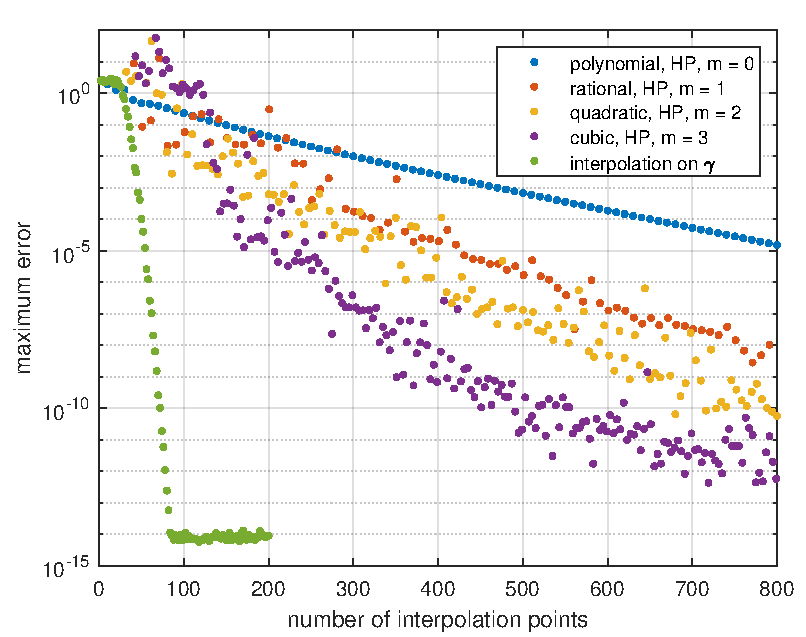
\includegraphics[width = 0.9\textwidth]{cubic_sing_ex.pdf}
	%\caption{   }   
	%\label{fig:convrates}
\end{figure}


\end{document}